%%%%%%%%%%%%%%%%%%%%%%%%%%%%%%%%%%%%%%%%%%%%%%%%%%%%%%%%%%%%%%%%%%%%%%%%%
% This file is part of the LaTeX sources of the OMDoc 1.3 specification
% Copyright (c) 2016 Michael Kohlhase.
% Source at https://github.com/KWARC/OMDoc/tree/master/doc/spec
% This work is licensed by the Creative Commons Share-Alike license
% see http://creativecommons.org/licenses/by-sa/2.5/ for details
%%%%%%%%%%%%%%%%%%%%%%%%%%%%%%%%%%%%%%%%%%%%%%%%%%%%%%%%%%%%%%%%%%%%%%%%%

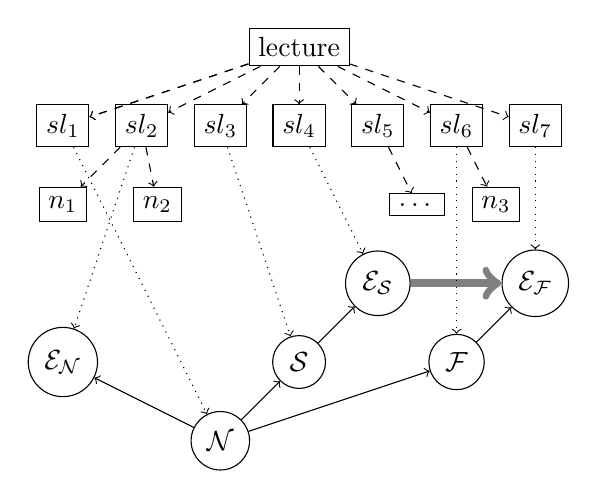
\begin{tikzpicture}
  \begin{scope}[shape=circle]
    \tikzstyle{every node}=[draw]
    \node (N)  at (2,0.5) {$\cal N$};
    \node (EN) at (0,1.5) {$\cal E_N$};
    \node (F)  at (5,1.5) {$\cal F$};
    \node (S)  at (3,1.5) {$\cal S$};
    \node (EF) at (6,2.5) {$\cal E_F$};
    \node (ES) at (4,2.5) {$\cal E_S$};
  \end{scope}
  \draw[->] (N) -- (EN);
  \draw[->] (N) -- (F);
  \draw[->] (N) -- (S);
  \draw[->] (S) -- (ES);
  \draw[->] (F) -- (EF);
  \draw[->,gray,line width=3pt] (ES) -- (EF);
  \begin{scope}
    \tikzstyle{every node}=[draw]
  \node (top) at (3,5.5) {lecture};
  \node (sl1) at (0,4.5) {$sl_1$};
  \node (sl2) at (1,4.5) {$sl_2$};
  \node (sl3) at (2,4.5) {$sl_3$};
  \node (sl4) at (3,4.5) {$sl_4$};
  \node (an) at (4,4.5) {$sl_5$};
  \node (sl5) at (5,4.5) {$sl_6$};
  \node (sl6) at (6,4.5) {$sl_7$};
  \node (n1) at (0,3.5) {$n_1$};
  \node (n2) at (1.2,3.5) {$n_2$};
  \node (n5) at (4.5,3.5){\ldots};
  \node (n6) at (5.5,3.5) {$n_3$};
\end{scope}
  \draw[->,dashed] (top) -- (sl1);
  \draw[->,dashed] (top) -- (sl1);
  \draw[->,dashed] (top) -- (sl2);
  \draw[->,dashed] (top) -- (sl3);
  \draw[->,dashed] (top) -- (sl4);
  \draw[->,dashed] (top) -- (an);
  \draw[->,dashed] (top) -- (sl5);
  \draw[->,dashed] (top) -- (sl6);
  \draw[->,dashed] (sl2) -- (n1);
  \draw[->,dashed] (sl2) -- (n2);
  \draw[->,dashed] (an) -- (n5);
  \draw[->,dashed] (sl5) -- (n6);

  \draw[->,dotted] (sl1) -- (N);
  \draw[->,dotted] (sl2) -- (EN);
  \draw[->,dotted] (sl3) -- (S);
  \draw[->,dotted] (sl4) -- (ES);
  \draw[->,dotted] (sl5) -- (F);
  \draw[->,dotted] (sl6) -- (EF);
\end{tikzpicture}

%%% Local Variables: 
%%% mode: latex
%%% TeX-master: "omdoc"
%%% End: 

% LocalWords:  EF sl
